\documentclass[10pt]{article}
\usepackage[letterpaper,margin=0.75in,headheight=14pt]{geometry}
\usepackage[utf8]{inputenc}
\usepackage[T1]{fontenc}
\usepackage{amsmath,amssymb,amsfonts}
\usepackage{booktabs}
\usepackage{graphicx}
\usepackage{float}
\usepackage{fancyhdr}
\usepackage{microtype}
\usepackage{nicefrac}
\usepackage{caption}
\usepackage{xcolor}
\usepackage{tabularx}
\usepackage{array}
\usepackage{enumitem}
\setlist{nosep}
\usepackage[compact]{titlesec}
\usepackage{url}
\usepackage[colorlinks=true,linkcolor=black,citecolor=black,urlcolor=blue]{hyperref}
\usepackage{algorithm}
\usepackage[noend]{algpseudocode}
\graphicspath{{figures/}}
\captionsetup{font=small,labelfont=bf,skip=4pt}
\captionsetup[table]{position=top}
\titlespacing*{\section}{0pt}{1.6ex plus .4ex minus .2ex}{0.8ex plus .2ex}
\titlespacing*{\subsection}{0pt}{1.2ex plus .3ex minus .2ex}{0.5ex plus .1ex}
\titlespacing*{\paragraph}{0pt}{0.6ex plus .2ex}{0.8em}
\renewcommand{\topfraction}{0.85}
\renewcommand{\bottomfraction}{0.6}
\renewcommand{\textfraction}{0.12}
\renewcommand{\floatpagefraction}{0.8}
\setcounter{topnumber}{3}
\setcounter{totalnumber}{4}
\urlstyle{same}
\setlength{\textfloatsep}{8pt plus 1pt minus 1pt}
\setlength{\floatsep}{8pt plus 1pt minus 1pt}
\setlength{\intextsep}{8pt plus 1pt minus 1pt}
\pagestyle{fancy}
\fancyhf{}
\renewcommand{\headrulewidth}{0pt}
\fancyhead[L]{MARL for Adversarial Spatial Decision-Making}
\fancyfoot[C]{\thepage}
\newcommand{\Wallz}{\textbf{Modified Wallz}}
\title{\vspace{-2.2em}Multi-Agent Reinforcement Learning for Adversarial Spatial\\ Decision-Making with Temporal Constraints\\[0.4ex]
\large Final Project Report}
\author{Vedant Bondekar, Abhishek Tagalpallewar, Chaitanya Chaudhary, Dhruv Meshram\\
Indian Institute of Technology Gandhinagar\\
\texttt{\{vedant.bondekar, abhishek.tagalpallewar,}\\
\texttt{chaitanya.chaudhary, dhruv.meshram\}@iitgn.ac.in}}
\date{November 22, 2026\vspace{-1.2em}}

\begin{document}
\maketitle
\thispagestyle{empty}

\begin{abstract}
We study \Wallz{}, a turn-based, two-player zero-sum Markov game extending wall-placement mechanics with reusable walls (A), a one-time hop (B), and temporary cell blocking (C). We implement a unified rule engine and four agents: shortest-path heuristic, depth-limited Minimax with Alpha-Beta pruning, an exact retrograde solver, and masked negamax Double-DQN trained via self-play. On miniature boards, the solver determines exact minimax values for up to 462{,}606 states; DQN selects value-preserving actions in 96\% of non-terminal states. In a paired $2^3$ factorial ablation on $5\times5$ (40 distinct 4-ply openings), only the hop has a Holm-significant effect on match outcomes, whereas reusable walls and blocks increase branching by 136\% and 46\%, reducing Minimax search depth by 2.0 and 0.6 plies. Self-play DQN defeats the heuristic in 78\% of distinct games on $5\times5$ but 50\% on $9\times9$. Of the proposed hypotheses, H1 holds, H3 holds on $4\times4$ and, at the proposal's $5\times10^5$-step budget, on $3\times3$, and H2 and H4 are refuted.
\end{abstract}

\noindent\textbf{Keywords:} Multi-Agent Reinforcement Learning, Deep Q-Network, Self-Play, Zero-Sum Games, Retrograde Analysis, Alpha-Beta Pruning, Legal-Action Masking

\section{Introduction}
In turn-based spatial games, wall placements alter navigable graph topology, dynamically shifting legal action spaces and position evaluations. \Wallz{} is a sequential zero-sum Markov game of perfect information where pawns race to opposite goal rows on an $N\times N$ grid under path preservation. We extend standard mechanics with three features: (A)~\emph{reusable walls}, repositioning a player's most recent wall; (B)~a \emph{one-time hop} across an opponent wall; and (C)~\emph{temporary cell blocking} for $K$ plies. Implementation and results are in our repository (\url{https://github.com/vedantb7/FAI_project.git}, Section~\ref{sec:repo}).

We investigate three research questions: \textbf{(RQ1)} how temporary and reusable constraints affect search and learning; \textbf{(RQ2)} how a one-time bypass alters planning; and \textbf{(RQ3)} how value-based MARL scales vs.\ exact values. We test four hypotheses in Section~\ref{sec:results}:
\textbf{H1}: A and C each raise branching by $\geq 40\%$ and reduce Minimax depth under fixed time;
\textbf{H2}: DQN with heuristic warm-up achieves $\geq 75\%$ wins vs.\ heuristic within $2\times10^5$ steps, vs.\ $\leq 55\%$ for pure self-play;
\textbf{H3}: mean value error on solvable boards ($N\leq 4$) falls below $0.15$;
\textbf{H4}: combined mechanics lengthen games beyond the sum of individual effects.

Positioned in course directions C (known rules vs.\ learned values) and D (search and learning under budget constraints), our contributions are: (i) a single verified rule engine shared by all agents, solver, and web demo; (ii) an exact retrograde solver for cyclic game graphs; (iii) a paired factorial evaluation over distinct openings; and (iv) an empirical comparison of heuristic, search, exact, and MARL agents on boards from $3\times3$ to $9\times9$.

\section{Problem Formulation}\label{sec:formulation}\subsection{Game model}
\Wallz{} is a finite, deterministic, two-player zero-sum Markov game of perfect information~\cite{littman1994,sutton2018} $\mathcal{G}=\langle \mathcal{N},\mathcal{S},(\mathcal{A}_i)_{i\in\mathcal{N}},T,(R_i)_{i\in\mathcal{N}},\gamma,s_0,\mathcal{S}_{\text{term}}\rangle$ with players $\mathcal{N}=\{1,2\}$ and turn indicator $z_t$. The board is $C=\{1,\dots,N\}^2$ with goal rows $G_1$ (top) and $G_2$ (bottom). Wall $w=(c,o)$, $o\in\{\mathrm{H},\mathrm{V}\}$, removes edge set $E(w)$. With $d_i(s)$ shortest-path distance to goal, $\mathrm{PathExists}(s,i)=\mathbb{I}[d_i(s)<\infty]$ and heuristic $H_i(s)=d_{-i}(s)-d_i(s)$.

\paragraph{State.} We extend state representations with operational counters:
\begin{equation}
s_t=\big(p_1,p_2,\;W_{1,t},W_{2,t},\;r_1,r_2,\;m_1,m_2,\;h_1,h_2,\;b_1,b_2,\;\tau_t,\;z_t\big),
\end{equation}
tracking player walls $W_{i,t}$, latest wall $r_i$, inventory $m_i\in\{0,\dots,M\}$, flags $h_i,b_i\in\{0,1\}$, and block timers $\tau_t:C\to\{0,\dots,K\}$. Wall ownership is tracked as hops only cross opponent walls.

\paragraph{Actions.} The active player $i=z_t$ selects an action from $\mathcal{A}_i(s)=\mathcal{A}^{\text{move}}_i\cup\mathcal{A}^{\text{place}}_i\cup\mathcal{A}^{\text{replace}}_i\cup\mathcal{A}^{\text{hop}}_i\cup\mathcal{A}^{\text{block}}_i$:
\begin{itemize}[leftmargin=1.5em]
\item \textbf{Move:} one orthogonal step across an open edge to an unblocked, unoccupied cell.
\item \textbf{Place:} legal iff $m_i>0$, wall does not overlap/cross existing walls, and $\mathrm{PathExists}(s\oplus w,j)=1$ for both $j$; sets $m_i'=m_i-1$ and $r_i'=w$.
\item \textbf{Replace (A):} repositions $r_i$ to free slot $w'$ at zero inventory cost, preserving both paths.
\item \textbf{Hop (B):} legal iff $h_i=1$, adjacent cell $c'$ is closed by an opponent wall $\{p_i,c'\}\in E(W_{-i,t})$, $\tau_t(c')=0$, $c'\neq p_{-i}$, and $\mathrm{PathExists}=1$; sets $h_i'=0$.
\item \textbf{Block (C):} legal iff $b_i=1$, $c^*$ is empty/unblocked, and paths survive without $c^*$; sets $b_i'=0$.
\end{itemize}
Transitions follow proposal rules: $\tau_{t+1}(c^*)=K$ for new blocks and $\tau_{t+1}(c)=\max(0,\tau_t(c)-1)$ otherwise. All actions are verified against $\mathcal{A}_i(s)$ before application.

\paragraph{Terminal states and rewards.} Reaching a goal row yields $R_i=+1, R_{-i}=-1$. Because boxed-in pawns may have no legal moves (48 such terminal states exist in $3\times3, M=1$), we define $\mathcal{A}_{z}(s)=\emptyset$ as a \emph{draw}, and declare draws on 5-fold repetition. Games reaching $T_{\max}=200$ plies are marked \emph{truncated}. Draws and truncations give $R_1=R_2=0$. The solution concept is the undiscounted minimax value $V^*(s)\in\{\text{WIN},\text{DRAW},\text{LOSS}\}$; $\gamma$ is used only by the DQN (Section~\ref{sec:method}). The repetition rule depends on the position history, which $s_t$ does not record: the engine keeps the history alongside $s_t$, and the solver solves the history-free position game (Section~3.4).

\subsection{Deviations from the proposal}
Table~\ref{tab:dev} details changes from the proposal. Crucially, the 2-cell hop was revised to a 1-cell step across opponent walls because the original rule yielded forced wins in 2--5 plies on all miniature boards. All reported results use the frozen final rules.

\begin{table}[!tb]
\centering\small
\caption{Main deviations from the submitted proposal and their reasons.}
\label{tab:dev}
\begin{tabular}{>{\raggedright\arraybackslash}p{4.2cm}>{\raggedright\arraybackslash}p{4.6cm}>{\raggedright\arraybackslash}p{6.3cm}}
\toprule
Proposal & Final & Reason\\
\midrule
Hop: 2-cell jump over a wall or pawn & 1-cell step across an opponent's wall & The jump made every miniature game a forced win in 2--5 plies\\
Binary outcomes only & Draw on no legal action and on 5-fold repetition & Such positions exist and some exact roots are infinite-play draws\\
Repeatable block & One block per player & Team rule decision; keeps the state finite and small\\
500 matches/pairing, 2-ply openings & Distinct openings only (Sec.~\ref{sec:protocol}) & Agents are deterministic: on $5\times5$ only 9 distinct 2-ply openings exist\\
DQN: 11 planes + 6 scalars, Adam $3\!\times\!10^{-4}$, warm-up & 14 planes, Adam $10^{-4}$, Double DQN, Huber loss; warm-up tested in H2 & Standard stabilisation; warm-up evaluated as an option\\
$5\times10^5$ steps $\times$ 5 seeds on every board & 5 seeds on $3\times3$ (200k; retrained to 500k for H3 only); one seed on $4\times4$ (500k), $5\times5$ (2M), $9\times9$ (5M) & Compute: one $9\times9$ run takes more than a day on a laptop CPU\\
\bottomrule
\end{tabular}
\end{table}

\section{Methodology}\label{sec:method}
All components share \texttt{wallz\_engine.py} as the sole rule implementation. Agents, solver, and web demo query legal actions and transitions directly from it; an AST test confirms no module duplicates rules.

\subsection{Rule engine and verification}
The engine generates $\mathcal{A}_i(s)$, validates path preservation via BFS only when placed assets intersect current shortest paths, applies moves transactionally, and exposes immutable position keys. Search nodes share repetition history copy-on-write; search planning is strictly deterministic. The engine was frozen after 35 dedicated unit tests covering block expiry, draws, wall inventories, and hop legality. Fuzzing executed 10{,}938 random plies and 3{,}235 hop-biased hops without error. All 454 tests pass.

\subsection{Tier 1: Greedy heuristic}
The heuristic agent evaluates legal actions by one-ply lookahead, maximising lexicographically
\begin{equation}
a^*=\arg\max_a \big(H_i(T(s,a)),\ \mathrm{cat}(a),\ -d_i(T(s,a)),\ -\mathrm{idx}(a)\big),
\end{equation}
executing immediate wins and assigning $H=0$ to terminal draws to prefer draws over losses. Category order (move $>$ replace $>$ hop $>$ wall $>$ block) is compared against the proposal tie order in Section~\ref{sec:results}.

\subsection{Tier 2: Minimax with Alpha-Beta pruning}
Minimax uses negamax with fail-hard Alpha-Beta pruning~\cite{knuth1975}:
\begin{equation}
V(s,d)=\begin{cases}\pm(1000-\text{ply}) \text{ or } 0 & s \text{ terminal (win/loss or draw)},\\ U_i(s)=\tanh\!\big(0.2\,H_i(s)\big) & d=0,\\ \max_{a\in\mathcal{A}_i(s)} -V\big(T(s,a),d-1\big) & \text{otherwise.}\end{cases}
\end{equation}
Monotone $\tanh$ bounds leaf scores below terminal payoffs; $-\text{ply}$ prefers faster wins. Moves are ordered by PV move, winning steps, pawn progress, path-cutting walls, other walls, and blocks, using history heuristics. Under time budgets, iterative deepening returns the best move of the deepest completed iteration. On 118 benchmark positions, Alpha-Beta replicates full-width minimax values while expanding up to $24\times$ fewer nodes (3{,}576 vs.\ 65{,}697 on twenty $5\times5$ positions at depth 2).

\textbf{Hop-aware evaluation.} Standard distance ignores hop bypasses. An optional evaluator computes $d_i$ by BFS over augmented states $(\text{cell}, h_i)$, crossing opponent walls once when $h_i=1$, matching exact search on 240 random positions.

\subsection{Tier 3: Exact retrograde solver}
For miniature boards, the solver enumerates reachable states breadth-first via engine queries. Canonical keys discard permanent wall order and merge wall owners once hops are spent (compressing 1{,}953 keys to 1{,}341 nodes without altering game values). The position game awards wins at goal rows, draws on empty action sets or infinite cycles (equivalent to 5-fold repetition since rank-optimal paths never repeat states).

Because cycles preclude topological backward induction, we employ attractor retrograde analysis~\cite{allis1994} (Algorithm~\ref{alg:retro}). A FIFO queue labels WIN states when any child is a LOSS, and LOSS states when all children are WINs, producing exact distance-to-outcome ranks. Unlabelled nodes on complete graphs are proved DRAWs. If caps are reached, unlabelled nodes remain UNKNOWN; proven WIN/LOSS labels remain sound.

\begin{algorithm}[!tb]
\caption{Cycle-aware retrograde solver (values for the side to move)}
\label{alg:retro}
\begin{algorithmic}[1]
\small
\State $G\gets$ reachable graph from $s_0$ via the engine; $\mathrm{cnt}[u]\gets$ number of distinct children of $u$
\State label goal terminals LOSS (rank 0) and enqueue them; label no-legal-action terminals DRAW
\While{queue $Q$ not empty}
  \State $v\gets Q.\mathrm{pop}()$
  \For{each unlabelled parent $u$ of $v$}
    \If{$v$ is LOSS} \State $u\gets$ WIN, rank $\mathrm{rank}(v)+1$; $Q.\mathrm{push}(u)$
    \Else \State $\mathrm{cnt}[u]\gets\mathrm{cnt}[u]-1$; \textbf{if} $\mathrm{cnt}[u]=0$ \textbf{then} $u\gets$ LOSS, rank $1+\max_{c}\mathrm{rank}(c)$; $Q.\mathrm{push}(u)$
    \EndIf
  \EndFor
\EndWhile
\State unlabelled nodes $\gets$ DRAW if $G$ is complete, else UNKNOWN
\end{algorithmic}
\end{algorithm}

Validation includes: 18 unit cases covering cycles, draws, block expiry, and hop rules; complete agreement with an independent DFS/value-iteration solver across three games; and mutation tests where broken engine rules triggered 3--4 test failures.

\subsection{Masked negamax Double-DQN with self-play}
\textbf{Observation \& Actions.} States are encoded from the mover's perspective as 14 $N\times N$ planes: pawn locations, walls, recent walls, block timers $\tau/K$, inventories $m_i/M$, and hop/block flags. The action space $|\mathcal{A}_{\text{enc}}(N)|=4(N-1)^2+N^2+8$ spans 33 ($3\times3$), 97 ($5\times5$), and 345 actions ($9\times9$). Legal action mask $\mathcal{M}(s,a)$ is generated by the engine~\cite{huang2022}; an audit of 5{,}952{,}580 action ids confirmed zero discrepancies. \textbf{Architecture \& Learning.} Four $3\times3$ conv layers (64 channels) feed a 256-unit MLP predicting Q-values. Rewards are $+1$ on winning moves and 0 otherwise. Negamax Double-DQN targets~\cite{mnih2015,vanhasselt2016} account for alternating turns:
\begin{equation}
y=r-\gamma\,(1-\mathrm{done})\;Q_{\theta^-}\!\Big(s',\ \arg\max_{a':\mathcal{M}(s',a')=1} Q_\theta(s',a')\Big),\qquad \gamma=0.99,
\end{equation}
trained with Huber loss, Adam ($10^{-4}$), batch 128, gradient clipping (10), target updates every 1{,}000 steps, and decaying $\varepsilon$-greedy exploration. \textbf{Self-play.} Episodes mix current network (50\%), snapshot pool refreshed every $2\times10^4$ steps (40\%), and Greedy (10\%)~\cite{silver2018}, with left--right reflectional symmetry on odd boards. \textbf{Model sets.} Two independently trained sets of the five $3\times3$ seeds (42--46, 200k steps) exist: the study models (\path{checkpoints/final/}) used for agreement with exact values (Section~4.1) and the five-seed match results, and the retrained released models (\path{final_dqn/overnight/}) used for H2, H3 and RQ1. Both keep the value in 95.8--96.7\% of non-terminal states.

\subsection{Evaluation protocol}\label{sec:protocol}
\textbf{Distinct openings.} Deterministic policies yield identical games from identical openings. Matches start with $k$ random pawn moves shared across all factorial cells; only distinct openings are executed across both player seats (e.g., 40 distinct 4-ply openings on $5\times5$).
\textbf{Metrics.} We report win/draw/truncation/loss rates with 95\% Wilson intervals, mean length, value/rank-optimal agreement rates with $V^*$, and discounted value error $|\max_a Q(s,a)-V^*_\gamma(s)|$ ($V^*_\gamma=\pm\gamma^{\,\mathrm{rank}-1}$, $\gamma=0.99$).
\textbf{Factorial analysis.} For factors $A,B,C\in\{-1,+1\}$, contrast effects $\mathrm{eff}(F)=\bar y_{F=+1}-\bar y_{F=-1}$ yield 3 main, 3 two-way, and 1 three-way interaction. 95\% CIs are estimated via 10{,}000 paired bootstrap resamples clustered by opening, with Holm-Bonferroni correction ($\alpha=0.05$).

\section{Results}\label{sec:results}\subsection{Exact values on miniature boards}
Table~\ref{tab:solve} summarizes exact retrograde solves ($K=1$). With $M=1$, outcome depends on A alone: player 1 wins without reusable walls, while enabling A produces infinite-play draws in all cells. At $M=2$, the hop is decisive: enabling B converts a draw into a player-1 win in 7 plies. On $3\times3$, C expands state space $12\times$ ($\log_{10}$ effect $+1.08$), versus $2.7\times$ for A and $3.4\times$ for B. Exact ground truth spans $N=3$ ($M\le 2$) and $N=4$ ($M\le 1$, C off); C-on cells on $4\times4$ exceeded the 400k-state cap, and 7 cells of $N=4, M=2$ exceeded $10^6$ states (reported as UNKNOWN).

\begin{table}[!tb]
\centering\small
\caption{Exact retrograde solves ($K=1$). Root value for player 1 with rank (plies to the result under optimal play).}
\label{tab:solve}
\begin{tabular}{lc>{\raggedright\arraybackslash}p{5.6cm}>{\raggedright\arraybackslash}p{3.9cm}r}
\toprule
Setting & Solved & Root value (player 1) & Note & Largest solved cell\\
\midrule
$N=3$, $M=0$ & 8/8 & WIN in 3 (C off), WIN in 5 (C on) & no walls: A, B inactive & 642 states\\
$N=3$, $M=1$ & 8/8 & WIN (rank 5--9) without A; DRAW with A & 48 no-move draws (A+B+C) & 150{,}710 states\\
$N=3$, $M=2$ & 8/8 & A off: DRAW (B off), WIN in 7 (B on); A on: DRAW & & 462{,}606 states\\
$N=4$, $M=0$ & 8/8 & LOSS in 6 (C off), LOSS in 8 (C on) & & 4{,}512 states\\
$N=4$, $M=1$ & 4/8 & LOSS (rank 10 / 8) without A; DRAW with A & C-on cells UNKNOWN (cap) & 372{,}160 states\\
$N=4$, $M=2$ & 1/8 & LOSS in 20 (all mechanics off) & 7 cells UNKNOWN (cap $10^6$) & 335{,}572 states\\
\bottomrule
\end{tabular}
\end{table}

\textbf{Agents vs.\ exact ground truth.} On 300 sampled states of $3\times3, M=1$ (all mechanics), value-optimal rates are 0.897 for Greedy, 0.953 for Minimax (d2), 0.967 for hop-aware Minimax, and 0.953--0.977 across five DQN seeds. Over all 138{,}646 non-terminal states, DQN preserves values in 96.0--96.6\% of states (rank-optimal 91.1--93.3\%, sign agreement 97.7--97.9\%). The $4\times4$ model ($M=0$, 4{,}350 states) preserves values in 96.3\% of states. Against the exact solver across 16 distinct openings and seats, every $3\times3$ DQN replicates exact game values (4 wins, 8 draws, 4 losses).

\subsection{Mechanics and search complexity (H1, H4)}
Figure~\ref{fig:branching} benchmarks 40 positions per cell on $5\times5$ ($K=3, M=10$) under Minimax (depth $\le 8$, 2.0\,s/move). Reusable walls increase mean branching from 14.7 to 34.5 ($+136\%$) and reduce completed depth from 6.35 to 4.28 plies. Blocks increase branching to 21.3 ($+46\%$), reducing depth by 0.6 plies. Hop affects neither ($+3\%$). Thus, \textbf{H1 holds} for A and C ($N=3, M=1$ exact solves show consistent trends: $+2.40$ actions for A, $+1.87$ for C). These are counts in the same fixed positions per cell. Averaged instead over the positions the ablation games reach (Section~4.3), every mechanic raises the mean legal-action count significantly, in a different order (C $+17.6$, B $+10.5$, A $+5.8$), because each cell's games pass through different positions; we did not separate the two effects.

H4 predicts super-additive game length. Factorial ablation reveals mean lengths: 24.1 (none), 41.9 (A), 15.3 (B), 26.2 (C), and 18.2 with all three active (vs.\ additive expectation 35.1 plies). \textbf{H4 is refuted}: hops bypass walls, producing a significant AB interaction on game length ($-6.0$ plies, $p<0.05$ Holm-corrected).

\begin{figure}[!tb]
\centering
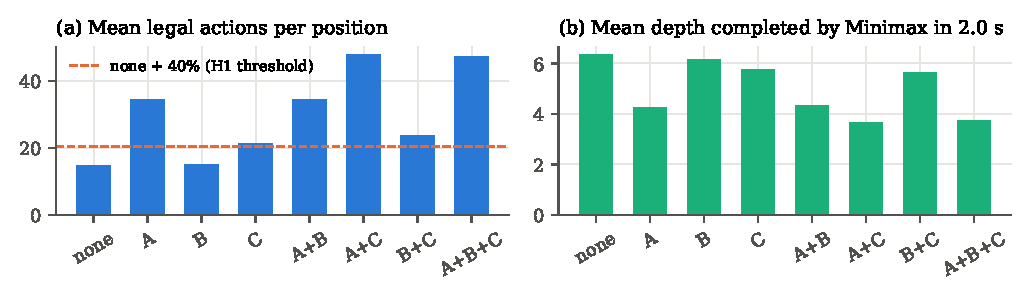
\includegraphics[width=0.76\textwidth]{branching.pdf}
\caption{H1 on $5\times5$, $K=3$, $M=10$ (40 positions per cell). (a) Mean legal actions; dashed line is the 40\% threshold above all-off cell. (b) Mean depth Minimax completes in 2.0\,s per move.}
\label{fig:branching}
\end{figure}

\subsection{Factorial ablation of the mechanics}
The $2^3$ ablation evaluates Minimax (d2) vs.\ Greedy across 8 cells on $5\times5$ from 40 distinct 4-ply openings in both seats (640 deterministic games, zero truncations). Figure~\ref{fig:ablation} reports win rates and effect sizes. \textbf{Only the hop exhibits a statistically supported effect}: it reduces Minimax win rate by 0.175 (95\% CI $[-0.259, -0.088]$), lowers draws by 0.122, and shortens games by 15.4 plies. Effects for A ($-0.081$) and C ($-0.037$) do not survive Holm correction (smallest effect detectable at 80\% power is $\approx 0.16$). With 2-ply (9 distinct) and 6-ply (40 distinct) openings the hop effect keeps its sign but is more than twice as large ($-0.40$ and $-0.41$), and with 6-ply openings C ($-0.088$) and the BC interaction ($+0.056$) also survive Holm correction. The size of the hop effect, and whether C is significant, therefore depend on the opening set; we did not establish why the 4-ply estimate is the smallest.

The hop dominates because default leaf evaluators overlook bypass opportunities: in the untimed Minimax d2 vs.\ Greedy match (Table~\ref{tab:matches}), 30 of Greedy's 60 wins used the hop. The hop-aware evaluator boosts Minimax win rate vs.\ Greedy by 11 points (39\% to 50\%, 95\% CI $[+1, +21]$) and wins 54\% head-to-head vs.\ default evaluation.

\begin{figure}[!tb]
\centering
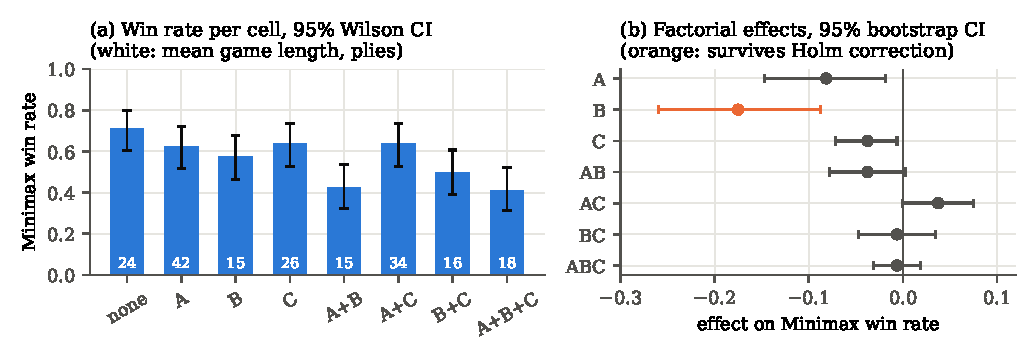
\includegraphics[width=0.78\textwidth]{ablation.pdf}
\caption{$2^3$ ablation, Minimax depth 2 vs.\ Greedy on $5\times5$, $K=3$, $M=10$; 80 distinct games per cell. (a) Win rate per cell. (b) Main effects and interactions; only B survives Holm correction.}
\label{fig:ablation}
\end{figure}

\subsection{Baselines on larger boards}
Table~\ref{tab:matches} presents match outcomes with all mechanics active ($K=3, M=10$). Greedy beats Random decisively (99.6\%), validating shortest-path heuristics. Untimed Minimax d2 wins only 39\% vs.\ Greedy on $5\times5$ due to unmodeled hops. Under a 2.0\,s budget, depth 4 reaches 54\% wins; depths 6 and 8 complete only about 4 plies on average (4.07 and 4.15) and play identical games (48\% wins each), so the time budget, not the nominal depth, sets practical strength. The proposal tie order (maximizing opponent distance) prioritized walls, winning fewer games vs.\ Random (488 vs.\ 498) and Minimax (47\% vs.\ 60\%), with 48\% truncated self-play on $9\times9$. We thus retain category priority as default.

\begin{table}[!tb]
\centering\small
\caption{Matches with all mechanics, $K=3$, $M=10$, both seats, distinct games only. W/D/T/L = win, rule draw, truncated, loss for the first-named agent. Openings: 50 distinct 4-ply openings on $5\times5$ and for the $9\times9$ DQN rows; 10 distinct 3-ply openings for $9\times9$ Greedy vs.\ Random. Games against Random repeat each opening and seat with several Random seeds.}
\label{tab:matches}
\begin{tabular}{llrcc}
\toprule
Board & Pairing & Games & W / D / T / L & Win \% [95\% Wilson]\\
\midrule
$5\times5$ & Greedy vs.\ Random & 500 & 498 / 1 / 0 / 1 & 99.6 [98.6, 99.9]\\
$5\times5$ & Minimax d2 (no limit) vs.\ Greedy & 100 & 39 / 1 / 0 / 60 & 39.0 [30.0, 48.8]\\
$5\times5$ & Minimax d2, hop-aware vs.\ Greedy & 100 & 50 / 2 / 0 / 48 & 50.0 [40.4, 59.6]\\
$5\times5$ & Minimax d4, 2.0\,s/move vs.\ Greedy & 100 & 54 / 5 / 0 / 41 & 54.0 [44.3, 63.4]\\
$5\times5$ & Minimax d8, 2.0\,s/move vs.\ Greedy & 100 & 48 / 11 / 0 / 41 & 48.0 [38.5, 57.7]\\
$5\times5$ & DQN (2M steps) vs.\ Greedy & 100 & 78 / 16 / 0 / 6 & 78.0 [68.9, 85.0]\\
$5\times5$ & DQN (2M steps) vs.\ Minimax d2 & 100 & 74 / 4 / 0 / 22 & 74.0 [64.6, 81.6]\\
$9\times9$ & Greedy vs.\ Random & 100 & 100 / 0 / 0 / 0 & 100.0 [96.3, 100.0]\\
$9\times9$ & DQN (5M steps) vs.\ Greedy & 100 & 50 / 41 / 0 / 9 & 50.0 [40.4, 59.6]\\
$9\times9$ & DQN (5M steps) vs.\ Minimax d2 & 100 & 56 / 5 / 7 / 32 & 56.0 [46.2, 65.3]\\
\bottomrule
\end{tabular}
\end{table}

\subsection{Learned policies: strength and convergence (RQ3, H2, H3)}
Figure~\ref{fig:dqn} summarizes DQN performance. On $3\times3$ (5 seeds), DQN wins 65\% vs.\ Greedy (SD 0.056) with 12.5\% losses. On $5\times5$, it wins 78\% vs.\ Greedy and 74\% vs.\ Minimax. On $9\times9$ (5M steps), performance declines to 50\% wins (41\% draws) vs.\ Greedy, and 39\% vs.\ proposal-order Greedy. A representation bottleneck exists: the 14-plane state encodes recent wall ownership but not older walls, altering hop legality in 14.6\% of $5\times5$ positions. Masks enforce legality, but value predictions lack full ownership context on larger boards. The trained $3\times3$ ($M=1$) and $4\times4$ ($M=0$) games are unaffected.

\begin{figure}[!tb]
\centering
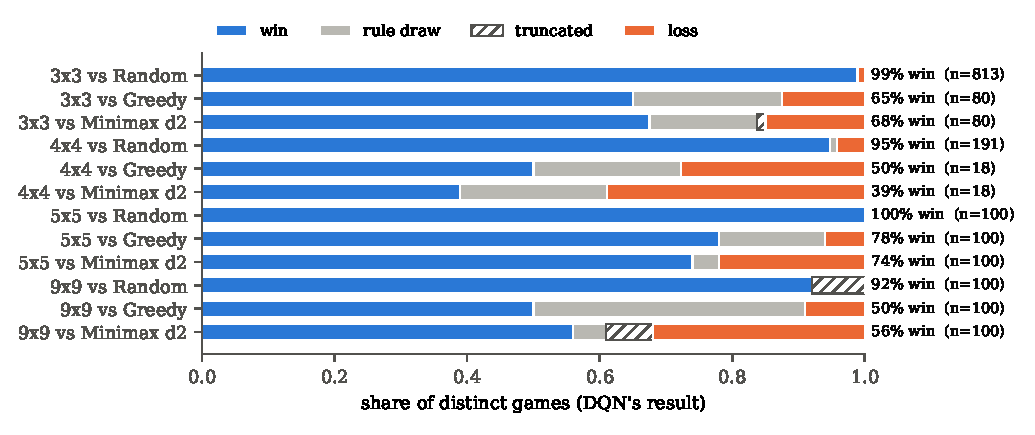
\includegraphics[width=0.78\textwidth]{dqn_boards.pdf}
\caption{DQN results by board and opponent over distinct games ($3\times3$: five seeds pooled; $4\times4$: one seed, 500k steps; $5\times5$: 2M; $9\times9$: 5M steps).}
\label{fig:dqn}
\end{figure}

\begin{figure}[!tb]
\centering
\begin{minipage}[c]{0.40\textwidth}
\centering
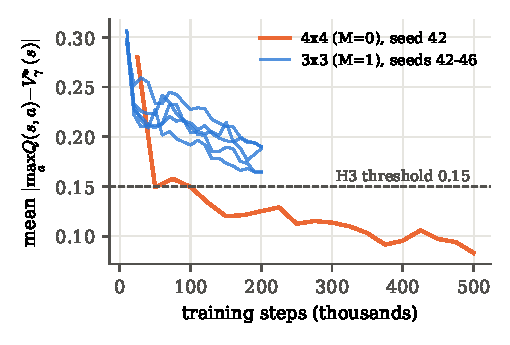
\includegraphics[width=\linewidth]{convergence.pdf}
\end{minipage}\hfill
\begin{minipage}[c]{0.56\textwidth}
\caption{H3: value error $|\max_a Q(s,a)-V^*_\gamma(s)|$ of every saved checkpoint over all non-terminal states of the exact solve. $4\times4$ ($M=0$, seed 42) falls below the 0.15 threshold from 100k steps and ends at 0.083; the five $3\times3$ ($M=1$) 200k-step seeds end at 0.164--0.190. The $3\times3$ 500k-step runs (text) are not plotted.}
\label{fig:h3}
\end{minipage}
\end{figure}

\textbf{H3.} Evaluating checkpoints against exact ground truth (Figure~\ref{fig:h3}), $4\times4$ error drops to 0.149 at 50k steps, briefly reaches 0.158 at 75k, stays below 0.15 from 100k, and ends at 0.083 ($<0.15$). On $3\times3$, errors finish at 0.164--0.190 at 200k steps, still falling on four of five seeds. Because 200k is below the proposal's $5\times10^5$-step budget, the five seeds were retrained from scratch to 500k steps (new trajectories, same configuration): all five end below 0.15 (0.114--0.145, mean 0.124), first crossing it at 311k--401k steps and staying below from 341k--481k. Hence, \textbf{H3 holds on $4\times4$ and, at the full budget, on $3\times3$}; it fails on $3\times3$ at 200k steps. The 150{,}710-state $3\times3$ game needs more training than the 4{,}512-state $4\times4$ game. All other $3\times3$ results use the 200k models.

\textbf{H2.} H2 compares opponent schedules on $3\times3$ (seed 42, 200k steps, Table~\ref{tab:h2rq1}, top). The match test cannot separate the arms: Greedy and the DQN are deterministic and the 200 evaluation games contain only 16 distinct games (8 distinct 2-ply openings $\times$ 2 seats), and all three arms score the same on them (10 wins, 4 draws, 2 losses; 62.5\% [38.6, 81.5]). The warm-up arm therefore does not reach 75\%, and pure self-play is not held to $\leq 55\%$. The value error separates the arms, against the hypothesis: warm-up has the highest (0.225 vs.\ 0.164--0.168). \textbf{H2 is refuted.}

\textbf{RQ1 for learning.} Across $3\times3$ cells (Table~\ref{tab:h2rq1}, bottom), reusable walls reduce value error across all 4 matched pairs (by 0.04--0.14), while cell blocks increase error (by 0.05--0.10), both exceeding the spread across five seeds (0.026).

\begin{table}[!tb]
\centering\small
\caption{DQN on $3\times3$, $K=1$, $M=1$, seed 42, 200k steps. Top: H2 opponent schedules. Bottom: one model per mechanics cell (RQ1). Value error is $|\max_a Q-V^*_\gamma|$ over all non-terminal states. W/D/T/L vs.\ Greedy over the 16 distinct games among 200 played (8 distinct openings $\times$ 2 seats), recovered from the stored per-seat counts and the known repeat count of each opening; for ``none'' two splits fit.}
\label{tab:h2rq1}
\setlength{\tabcolsep}{4pt}
\begin{tabularx}{\textwidth}{l>{\raggedright\arraybackslash}Xrrc}
\toprule
Run & Setting & Value-optimal & Value error & vs.\ Greedy W/D/T/L\\
\midrule
H2 warm-up & first $10^4$ learner moves from Greedy & 95.2\% & 0.225 & 10/4/0/2\\
H2 default & 50\% self, 40\% snapshots, 10\% Greedy & 95.8\% & 0.164 & 10/4/0/2\\
H2 pure self-play & 50\% self, 50\% snapshots & 96.4\% & 0.168 & 10/4/0/2\\
\midrule
RQ1 none & 1{,}341 states & 98.7\% & 0.183 & 11--12/2--3/0/2\\
RQ1 C & 16{,}696 states & 95.8\% & 0.236 & 10/0/0/6\\
RQ1 B & 4{,}893 states & 99.3\% & 0.130 & 12/0/0/4\\
RQ1 B+C & 59{,}240 states & 96.9\% & 0.234 & 10/2/0/4\\
RQ1 A & 3{,}861 states & 99.3\% & 0.049 & 6/8/0/2\\
RQ1 A+C & 46{,}886 states & 98.4\% & 0.097 & 6/8/0/2\\
RQ1 A+B & 12{,}821 states & 98.2\% & 0.088 & 12/2/0/2\\
RQ1 A+B+C (seeds 42--46) & 150{,}710 states & 95.8--96.7\% & 0.164--0.190 & 10--11/3--4/0/2\\
\bottomrule
\end{tabularx}
\end{table}

\section{Discussion and Limitations}
\textbf{The three mechanics act on different things (RQ1, RQ2).} Reusable walls and blocks increase search complexity, doubling branching and costing Minimax up to two plies under fixed compute. On small boards, reusable walls turn every one-wall $3\times3$ game into a draw. The hop governs outcomes: it is the sole mechanic with a statistically supported effect on win rates, alters exact values once walls are plentiful, and yields an 11-point boost when incorporated into leaf evaluation. Together, mechanics shorten games rather than lengthening them as hops bypass walls.

\textbf{Learned versus exact values (RQ3).} With sparse terminal rewards and no transition model, self-play DQN selects value-optimal actions in 96\% of states across games up to 150{,}710 states, with error falling below 0.15 on $4\times4$ and, given the full 500k-step budget, on $3\times3$. Reusable walls make values easier to learn whereas blocks hinder learning. Heuristic warm-up provides no benefit. Small-board optimality does not scale directly: DQN dominates baselines on $5\times5$ but performs on par with Greedy on $9\times9$.

\textbf{Limitations.} (i)~Only $3\times3$ default configurations include five seeds; larger boards have one. (ii)~Ground truth is absent above $4\times4$. (iii)~Deterministic policies constrain sample diversity to distinct openings. (iv)~Timed search depends on compute load. (v)~Ablation focuses on Minimax d2 vs.\ Greedy. (vi)~DQN inputs omit older wall owners, impacting $5\times5$ and $9\times9$. (vii)~Solving larger miniature cells exceeds 3\,GB host RAM limits. (viii)~The block duration $K$ is never varied: all solves and DQN runs use $K=1$ and all matches $K=3$, so the temporal constraint is studied only as block on/off. (ix)~On $3\times3$, match tests against deterministic opponents rest on 16 distinct games, too few to separate training variants; value metrics over all states carry those comparisons.

\section{Conclusion}
We developed a verified engine for \Wallz{} and evaluated four agent paradigms: heuristic lookahead, Alpha-Beta Minimax, exact retrograde analysis, and self-play Double-DQN under a paired factorial design. Reusable walls and temporary blocks primarily increase search branching; one-time hops determine match outcomes; and their interaction contracts game lengths. Model-free DQN masters near-optimal play on solvable boards and outperforms baselines on $5\times5$, though scaling limits emerge on $9\times9$. Future work includes owner-aware observations, expanded seed evaluations, and hop-aware evaluation inside neural policies.

\section{Repository and Reproducibility}\label{sec:repo}
Code, results, and documentation are hosted at \url{https://github.com/vedantb7/FAI_project.git}. The \texttt{README.md} outlines environment setup, test suites, match execution, training pipelines, and the interactive web demo (Flask backend, React frontend). All reported values are extracted directly from committed logs in \path{experiments/results/}, each recording commit hash, command flags, seeds, and Python environment; the figures plot values from these files. Results from outdated rules are quarantined in \path{experiments/results/STALE.md} and excluded.

\section{Contribution}\label{sec:contribution}
Following the proposal idea review, the team reassigned modular responsibilities. Table~\ref{tab:contrib} details individual task assignments and fulfillment status.

\begin{table}[!htb]
\centering\footnotesize
\caption{Final task allocation and completion status.}
\label{tab:contrib}
\begin{tabularx}{\textwidth}{>{\raggedright\arraybackslash}p{3.3cm}>{\raggedright\arraybackslash}X>{\raggedright\arraybackslash}p{3.8cm}}
\toprule
Member & Assigned tasks & Fulfilled?\\
\midrule
Vedant Bondekar & Minimax search with Alpha-Beta pruning, leaf evaluation $U_i(s)$, move ordering, iterative deepening; validation on the final rules; hop-aware evaluator & Yes\\
Abhishek Tagalpallewar & Core game engine and legal-action generator, Greedy heuristic baseline, rule freeze and test suite, interactive web demo (game, arena, replays) & Yes\\
Chaitanya Chaudhary & Match runner and logging, state-graph builder, exact retrograde solver and its validation, agreement metrics, $2^3$ factorial ablation and statistics, multi-seed study, result tables & Yes; 4 of 8 $N=4$, $M=1$ cells exceed the state cap (reported as UNKNOWN)\\
Dhruv Meshram & Masked DQN (CNN+MLP), action codec, self-play training pipeline, replay buffer, training and evaluation on $3\times3$--$9\times9$, H2/H3/RQ1 runs & Yes; one seed above $3\times3$ (compute)\\
\bottomrule
\end{tabularx}
\end{table}

\begin{thebibliography}{9}\footnotesize\setlength{\itemsep}{0pt}\setlength{\parskip}{0pt}
\bibitem{littman1994} M.~L. Littman. Markov games as a framework for multi-agent reinforcement learning. In \emph{Proc.\ ICML}, pages 157--163, 1994.
\bibitem{mnih2015} V.~Mnih et al. Human-level control through deep reinforcement learning. \emph{Nature}, 518(7540):529--533, 2015.
\bibitem{vanhasselt2016} H.~van Hasselt, A.~Guez, and D.~Silver. Deep reinforcement learning with double Q-learning. In \emph{Proc.\ AAAI}, 2016.
\bibitem{huang2022} S.~Huang and S.~Onta\~n\'on. A closer look at invalid action masking in policy gradient algorithms. In \emph{Proc.\ FLAIRS}, 2022.
\bibitem{silver2018} D.~Silver et al. A general reinforcement learning algorithm that masters chess, shogi, and Go through self-play. \emph{Science}, 362(6419):1140--1144, 2018.
\bibitem{allis1994} L.~V. Allis. \emph{Searching for Solutions in Games and Artificial Intelligence}. PhD thesis, Vrije Universiteit Amsterdam, 1994.
\bibitem{knuth1975} D.~E. Knuth and R.~W. Moore. An analysis of alpha-beta pruning. \emph{Artificial Intelligence}, 6(4):293--326, 1975.
\bibitem{sutton2018} R.~S. Sutton and A.~G. Barto. \emph{Reinforcement Learning: An Introduction}. MIT Press, 2nd edition, 2018.
\end{thebibliography}

\end{document}